\chapter{Grundlagen}

% -----------
% --- VMs ---
% -----------

\section{Virtuelle Maschinen}
Als virtuelle Maschine (kurz VM) wird in der Informatik die Nachbildung eines Rechnersystems bezeichnet. Die virtuelle Maschine bildet die Rechnerarchitektur eines real in Hardware existierenden oder hypothetischen Rechners nach \cite{Sieg2007}. Den virtuellen Maschinen wird über den sogenannten Hypervisor oder auch Virtual Machine Monitor (VMM) ein komplettes System vorgespielt, sodass diese die zugeteilten Ressourcen für echte Hardware halten \cite{OSTEP}.\\

\begin{figure}[!ht] % see https://en.wikibooks.org/wiki/LaTeX/Floats,_Figures_and_Captions for placement parameters
  \centering
  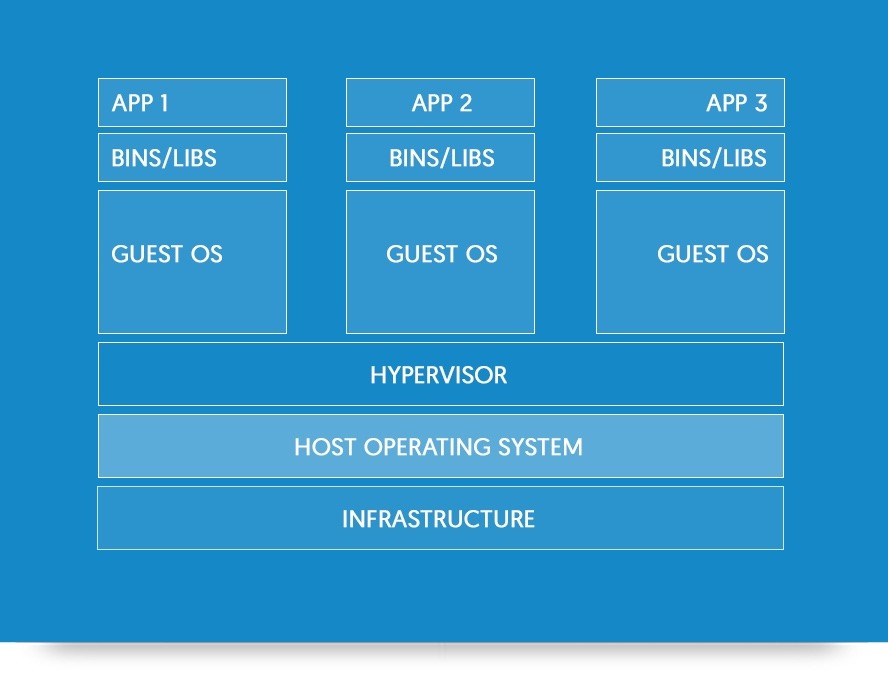
\includegraphics[width=0.5\textwidth]{images/docker-vm.jpg}
  \caption{Mehrere virtuelle Maschinen auf einem Host-System. \cite{docker}}
\end{figure}

Da neben der Applikation selbst noch eine ganze Reihe weiterer Ressourcen benötigt werden, nämlich das Betriebssystem und seine ungenutzte Bibliotheken führt dies zu höherem Ressourcenverbrauch und großen Abhängigkeiten vom Betriebssystem.\linebreak Zum Beispiel können bei einem Update des Betriebssystems für die Applikation nötige Bibliotheken verändert werden, die ein verändertes Verhalten hervorrufen. Dies bedeutet sowohl einen hohen Overhead an verbrauchten Systemressourcen, als auch einen hohen Wartungsaufwand.\\

\noindent Es wird meist zwischen Typ-1-Hypervisor und Typ-2-Hypervisor unterschieden. Inzwischen ließt man auch öfter von einem Typ-0-Hypervisor, einer neueren Technologie, auf die ich in dieser Arbeit nicht weiter eingehen werde.\\

\noindent Ein Typ-1-Hypervisor (native oder bare-metal) setzt direkt auf der Hardware auf und benötigt keine vorherige Betriebssystem-Installation, muss aber von der entsprechenden Hardware unterstützt werden.

\vspace{\baselineskip}

\noindent Ein Typ-2-Hypervisor (hosted) setzt auf einem vollwertigen Betriebssystem, auf dem Hostsystem, auf und nutzt die Gerätetreiber des Betriebssystems, um auf die Hardware des Hostsystems zuzugreifen. \cite{wiki:hyper}, \cite{6903537}\\

\begin{figure}[!ht] % see https://en.wikibooks.org/wiki/LaTeX/Floats,_Figures_and_Captions for placement parameters
  \centering
  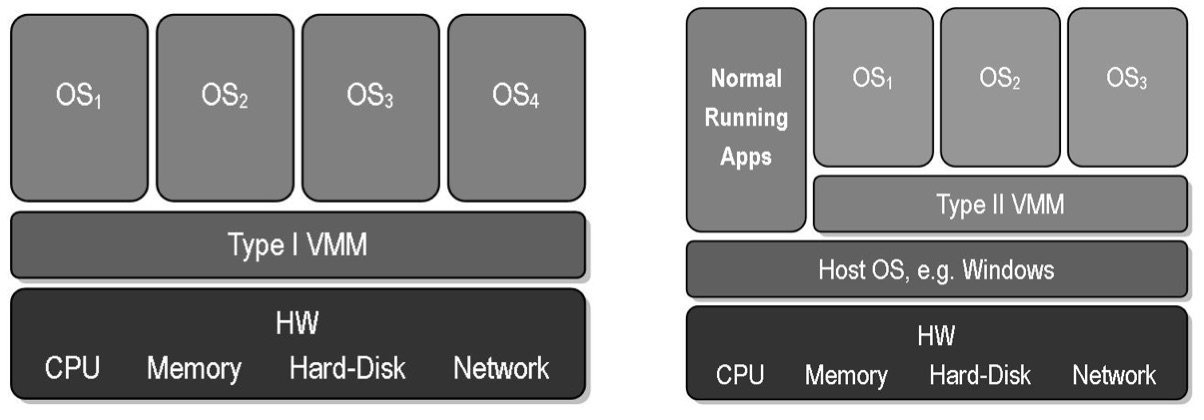
\includegraphics[width=0.8\textwidth]{images/hypervisors.jpg}
  \caption{Typ-1-Hypervisor und Typ-2-Hypervisor. \cite{wiki:hyper}}
\end{figure}

% ---------
% Container
% ---------

\section{Container}
Ein Gegenentwurf zu den virtuellen Maschinen sind sogenannte Container, die das Ziel haben mit weniger Overhead den gleichen Grad an Isolation und Sicherheit zu liefern.

\paragraph{}
Anders als virtuelle Maschinen, teilen sich Container das Betriebssystem mit dem Hostsystem auf dem die Container gestartet werden. Befehle können also nahezu direkt auf der Hardware ausgeführt werden und müssen nicht erst, wie bei den virtuellen Maschinen den Umweg über den Hypervisor gehen, was einen Performancevorteil mit sich bringt, schränkt die Container aber auch dahingehend ein, dass nur Anwendungen mit dem gleichen Kernel wie der Host gestartet werden können. So können also nicht nativ Windows Container in einer Linux-Umgebung gestartet werden und umgekehrt \cite{7092949}. Wie auch virtuelle Maschinen werden Container auf Basis von Images erstellt. Diese Container können gestoppt und gestartet werden.\\ Es gibt verschiedene Implementationen von Containern, aber die meisten basieren zumindest zu großen Teilen auf den folgenden Linux-Kernel Features, die ab Version 3.8 zur Verfügung standen \cite{RaRo}.

\paragraph{Chroot} \mbox{} \\
\noindent Chroot steht für „change root“ und ist eine Funktion unter Unix-Systemen, um das Rootverzeichnis zu ändern. Sie wirkt sich nur auf den aktuellen Prozess und seine Kindprozesse aus \cite{wiki:chroot}. So können die Container vom Dateisystem des Host-Systems isolieret werden.


\paragraph{Cgroups} \mbox{} \\
\noindent Cgroups (Control Groups) ermöglichen die Gruppierung von Prozessen, mit deren Hilfe das Betriebssystem den Gruppen Ressourcen zuweisen kann und verwalten kann. Control Groups können Ressourcen limitieren, priorisieren und isolieren. So kann man die Ressourcen für bestimmte Container limitieren und besser voneinander und dem Host-System isolieren \cite{7158965}.

\paragraph{Kernel Namespaces
} \mbox{} \\
\noindent Mit Hilfe Kernel Namespaces der Kernel Namespaces lassen sich Prozesse oder Gruppierungen von Prozessen auf verschiedenen Ebenen voneinander isolieren. Es gibt verschiedene Namespaces für unterschiedliche Zwecke:
\begin{itemize}
  \item pid um die Prozesse voneinander zu isolieren \cite{lnpid}
  \item net für eigene Netzwerk-Konfigurationen und Adressen \cite{lnnet}
  \item ipc für den Informations Austausch zwischen Containern \cite{lnipc}
  \item mnt für eigene Mountpoints \cite{lnns}
  \item uts für die Zuweisung eigener Hostnames \cite{lnuts}
\end{itemize}

\begin{figure}[!ht]
  \centering
  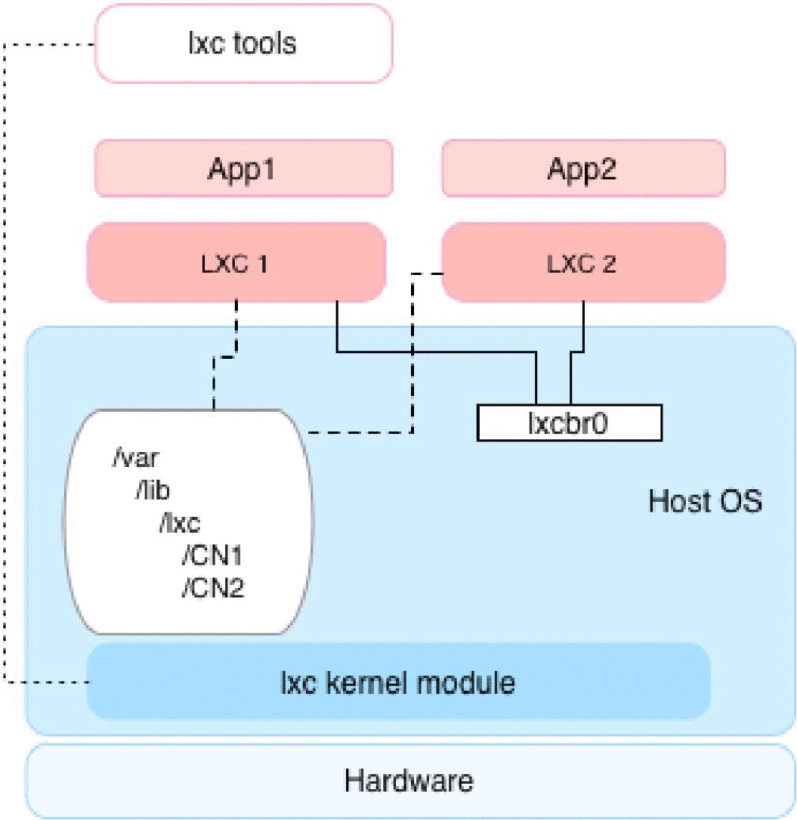
\includegraphics[width=0.5\textwidth]{images/containers.jpg}
  \caption{Containers \cite{6903537}}
\end{figure}

\paragraph{}
Es gibt verschiedene Ziele, die man mit einem Container erreichen will. Die zwei Hauptanwendungsfälle sind aber wohl OS-Container und Applikations-Container. Der Unterschied ist dabei aber kein technischer sondern mehr ein konzeptueller.\\
Ein OS-Container kann als virtuelle Maschine ohne Performance-Overhead betrachtet werden, die sich wie beschrieben den Kernel mit dem Host-System teilt. Die Container können, einmal gestartet, wie ein normales Betriebssystem bedient werden. Es können beliebig viele Container auf einem System laufen mit unterschiedlichsten Zielen. Zum Beispiel könnte man einen Container erstellen, auf dem man alle nötigen Services installiert, um eine Webanwendung laufen zu lassen. Lässt man den Container auf einem anderen Host-System laufen, sind wieder genau die gleichen Versionen der Programmiersprache, wie zB. Ruby oder PHP, der genutzten Datenbank oder dem Webserver aber auch von wichtigen System-Libraries, installiert. Genauso vorstellbar sind aber auch spezialisierte Container für Webserver und Datenbank, die über die Linux Bridge miteinander kommunizieren \cite{ocvsac}. Die einzelnen Prozesse für die jeweiligen Services werden dabei in den jeweiligen Containern gestartet und nicht auf dem Host-System. So kann sichergestellt werden, dass man auf unterschiedlichen Host-Systemen die gleiche Webanwendung immer auf den gleichen Maschinen laufen lässt.

\begin{figure}[!ht]
  \centering
  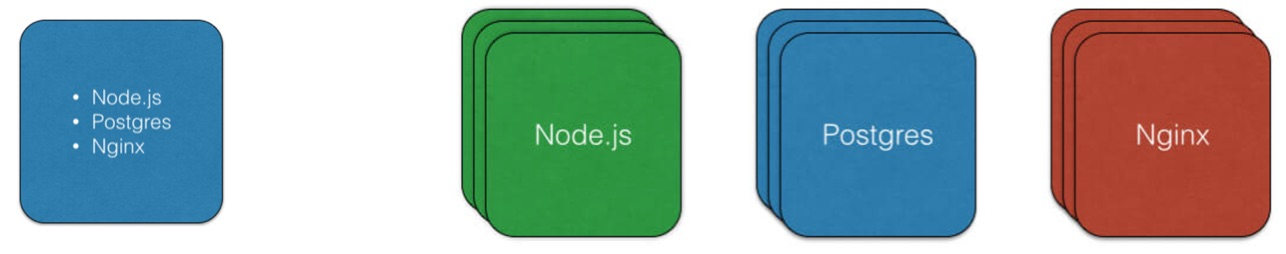
\includegraphics[width=0.8\textwidth]{images/os-specialized-containers.jpg}
  \caption{Ein OS-Container mit allen nötigen Servern vs. einzelne spezialisierte OS-Container}
\end{figure}

Im Gegensatz zu OS-Containern wird mit einem Applikations-Container das Ziel verfolgt, ein Paket mit allen nötigen Abhängigkeiten zu bauen, welches dann als einzelner Prozess gestartet werden kann.
Applikations-Container bestehen oft aus sogenannten Layern, einzelnen Images die später beim Bauen des Images, das zum starten der Anwendung verwendet wird zusammengefasst werden. Diese entsprechen den einzelnen spezialisierten Containern in dem oben genannten Beispiel. Der Vorteil ist, das die einzelnen Services in dem Fall im gleichen Namespace ausgeführt werden und dementsprechend aufeinander zugreifen können. Nutzt man Microservices als Architekturmuster ist es zum Beispiel sinnvoll, die einzelnen Services in Containern laufen zu lassen und die jeweiligen Layer in den verschiedenen Containern wiederzuverwenden.

\begin{figure}[!ht]
  \centering
  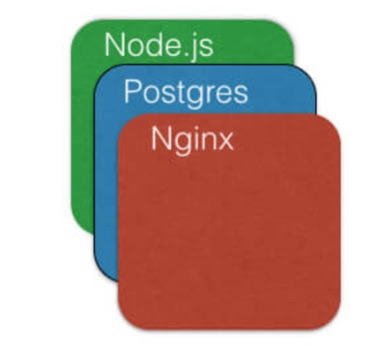
\includegraphics[width=0.4\textwidth]{images/application-container.jpg}
  \caption{Ein Applikations-Container mit mehreren Layern}
\end{figure}

% ---------
% Daemon
% ---------

\section{Daemon}
Als Daemon bezeichnet man unter Unix oder unixartigen Systemen ein Programm, das im Hintergrund abläuft und bestimmte Dienste zur Verfügung stellt. Der Benutzer interagiert dabei nicht direkt mit dem Programm, sondert indirekt über Ereignisse auf dem System. Das kann zum Beispiel eine Hardwareüberwachung sein, die überprüft ob ein Wechselmedium an das System angeschlossen wurden, aber auch ein Webserver, der auf Anfragen HTTP-Anfragen wartet \cite{wiki:daemon}.
